%%%%%%%%%%%%%%%%%%%%%%%%%%%%%%%%%%%%%%%%%%%%%%%%%%%%%%%%%%%%%%%%%%%%%%%%%%%%%%%%
%                                                                              %
%                     ELEN4009 - Software Engineering                          %
%                                                                              %
%                           Software Design                                    %
%                                 for                                          %
%         The Online Postgraduate Application Approval System for EIE          %
%                                                                              %
%             Julio Baeta (710066), Nomakhosi Ndebele (671480),                %
%             Ryan Robinson (453764),Timothy Rokebrand (458960)                %
%                                                                              %
%          This LaTeX document was adapted from the IEEE template,             %
%                           which can be found at:                             %
% http://www.ieee.org/conferences_events/conferences/publishing/templates.html %
%                                                                              %
%%%%%%%%%%%%%%%%%%%%%%%%%%%%%%%%%%%%%%%%%%%%%%%%%%%%%%%%%%%%%%%%%%%%%%%%%%%%%%%%

\documentclass[journal,comsoc,onecolumn]{IEEEtran}
\usepackage[T1]{fontenc}
\usepackage{fancyhdr}
\usepackage{graphicx}

%%%%%%%%%%%%%%%%%%%%%%%%%%%%%%%%%%%%%%%%%%%%%%%%%%%%%%%%%%%%%%%%%%%%%%%%%%%%%%%%

\begin{document}

%%%%%%%%%%%%%%%%%%%%%%%%%%%%%%%%%%%%%%%%%%%%%%%%%%%%%%%%%%%%%%%%%%%%%%%%%%%%%%%%

\title{Description of Demonstrable Modules \\ \vspace{7mm} for \\ \vspace{7mm} The Online Postgraduate Application \\ Approval System for EIE}

\author{\vspace{3mm} Julio Baeta (710066), Nomakhosi Ndebele (671480), Ryan Robinson (453764), Timothy Rokebrand (458960)\\ \small \vspace{2mm} School of Electrical \& Information Engineering, University of the Witwatersrand, Private Bag 3, 2050, Johannesburg, South Africa}

\markboth{}{}

\maketitle

\thispagestyle{empty}

%%%%%%%%%%%%%%%%%%%%%%%%%%%%%%%%%%%%%%%%%%%%%%%%%%%%%%%%%%%%%%%%%%%%%%%%%%%%%%%%

\newpage

\thispagestyle{empty}

\section{INTRODUCTION}
The following document gives a description of the modules developed thus far. These modules show the basic design of the proposed webpage, and also demonstrate the communication between the front-end and back-end in order to retrieve information from a database.

\section{LOGIN PAGE}
The first page is the login page, although not functional at this point in time this will be the first line of security when logging into the page.  In future versions the user will enter their personal details and this information will be used to determine who the user is and what level of access to  the page they have.

\begin{figure}[h]
\centering
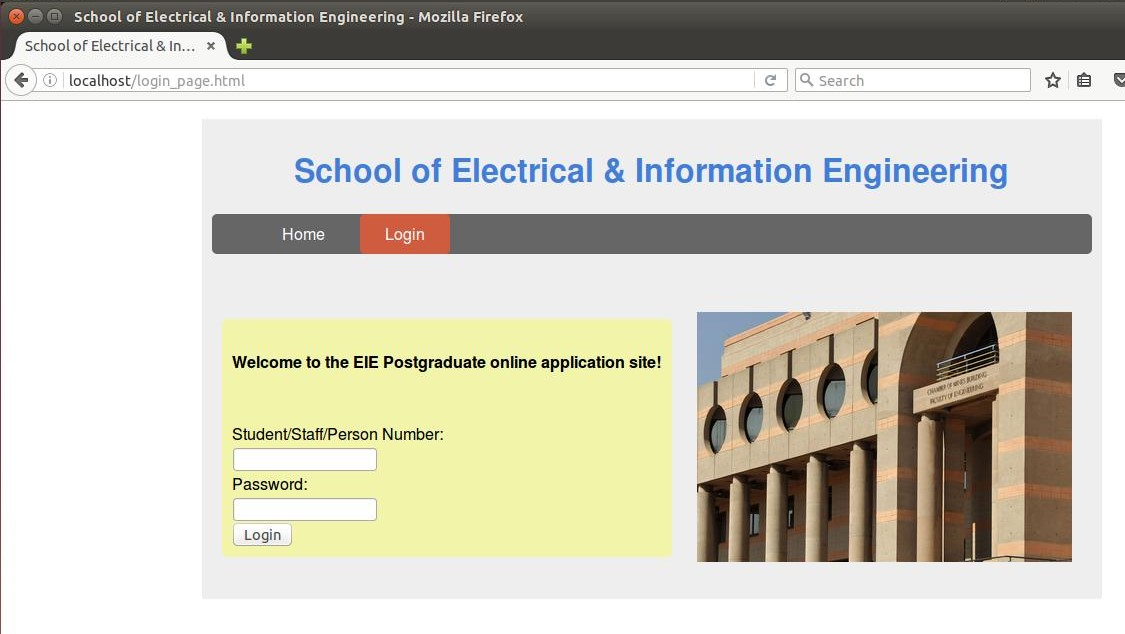
\includegraphics[width=0.7\linewidth]{loginpage}
\caption{Login Page}
\label{fig:loginpage}
\end{figure}

\section{HOME PAGE}
The next page is the home screen, extra information can be added in order to assist the user with the page and display any information that may be of use. The user will be able to navigate back to this page at any time. 

\begin{figure}[h]
	\centering
	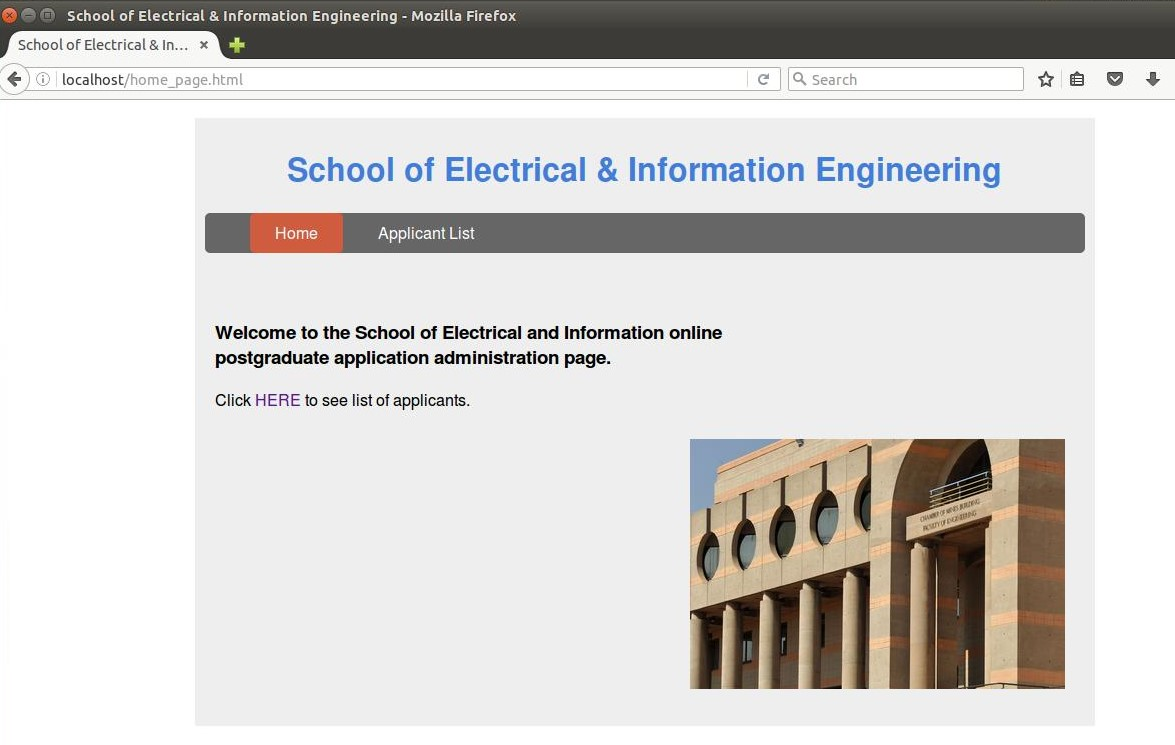
\includegraphics[width=0.7\linewidth]{home}
	\caption{Home Page}
	\label{fig:home}
\end{figure}
\section{APPLICANT LIST}
The Applicant list shows a list of applicants that are in the process of having their applications processed. This list is populated using the created MySQL database. This is acheived by using a unconditional select query which will acheive all the infomation form the students\_infomation table. In future versions this information will only be visible to respective supervisors. 

\begin{figure}[h]
\centering
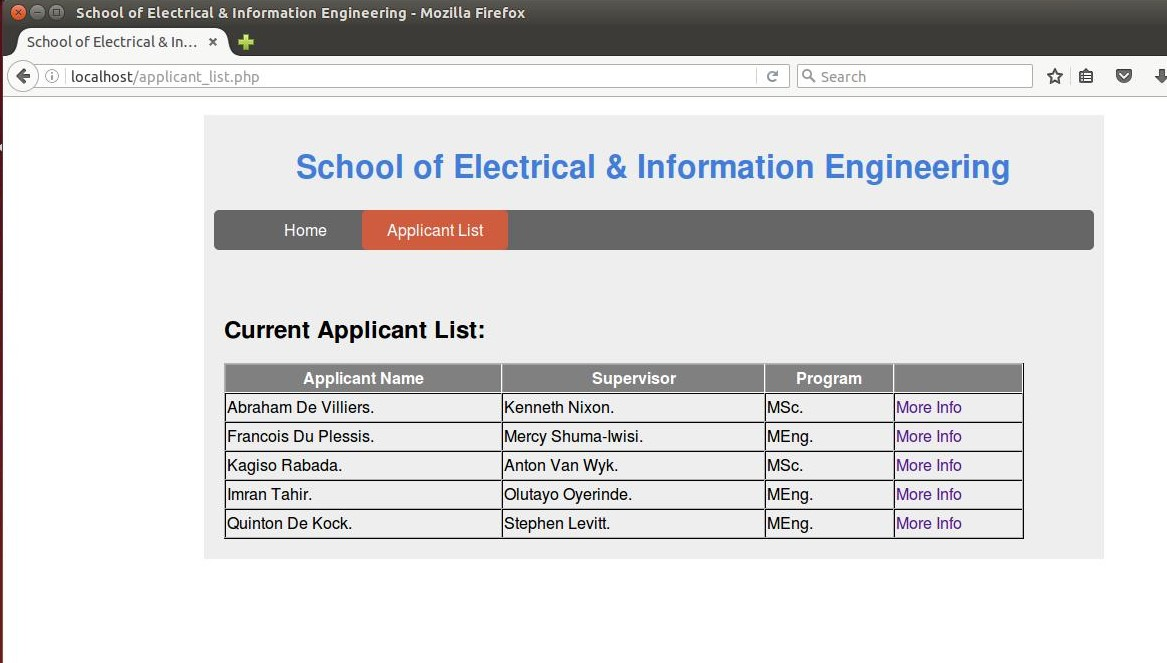
\includegraphics[width=0.7\linewidth]{list}
\caption{List Of All Applicants}
\label{fig:list}
\end{figure}

The student\_information table was created and then populated with insert query to look like below

\begin{figure}[h]
\centering
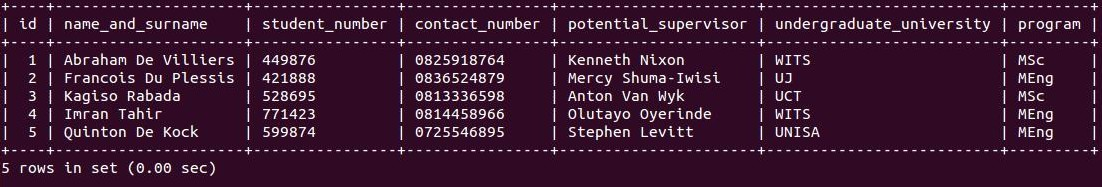
\includegraphics[width=0.7\linewidth]{mysql}
\caption{Student\_Information Table In My SQL}
\label{fig:mysql}
\end{figure}

\newpage
\section{APPLICANT INFORMATION}
When "More info" is selected the Applicant's information is displayed. The specific individual's is displayed; this is done by getting the relevant postgraduates id which is passed to the page though a GET request. The id is used to modify the select query for the database so that only the specific information is retrieved. 

\begin{figure}[h]
\centering
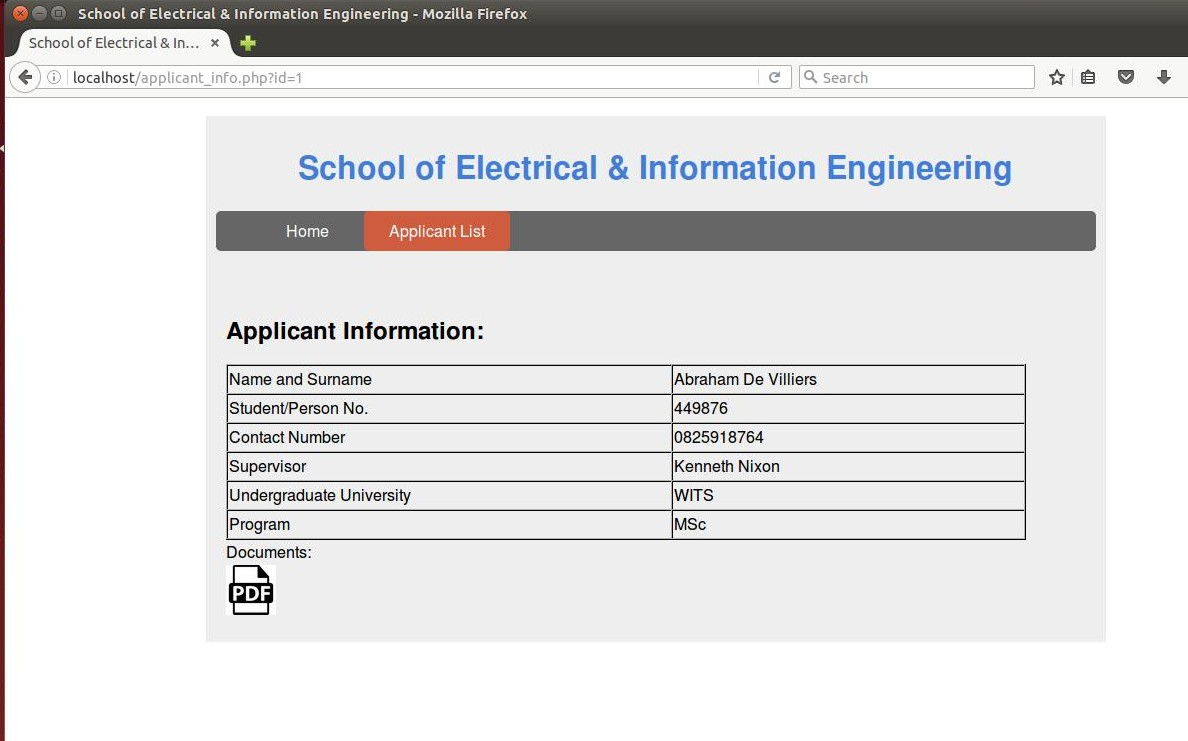
\includegraphics[width=0.7\linewidth]{information}
\caption{An Applicant's Information Page}
\label{fig:information}
\end{figure}





\section{FUTURE DEVELOPMENT}
In future versions the user will navigate from this page to a decisions page that will allow him/her to approve or reject the application and give comments on the decision. These comments will be passed to the back-end…..


\end{document}

%%%%%%%%%%%%%%%%%%%%%%%%%%%%%%%%%%%%%%%%%%%%%%%%%%%%%%%%%%%%%%%%%%%%%%%%%%%%%%%%